\documentclass[UTF8,fontset=fandol,11pt,a4paper]{ctexart}
\newcommand{\EnglishReport}{}
% Group information supplied for ECE2013, Fall 2026. No student IDs requested.
\newcommand{\CourseCode}{ECE2013}
\newcommand{\CourseTerm}{Fall 2026}
\newcommand{\GroupNumber}{6}
\newcommand{\GroupMembersZh}{王骊斌、蒋佳豪、王子征、薛晓康}
\newcommand{\GroupMembersEn}{Wang Libin, Jiang Jiahao, Wang Zizheng, Xue Xiaokang}

\newcommand{\CourseName}{Advanced AI Algorithms and Systems}
\newcommand{\ReportDate}{November 5, 2026}
\usepackage{assignment}
\newcommand{\DesignedGames}{40}
\newcommand{\DesignedWins}{40}
\newcommand{\DesignedLosses}{0}
\newcommand{\DesignedDraws}{0}
\newcommand{\DesignedWinRate}{100.0\%}
\newcommand{\DesignedMeanNodes}{6,516.7}
\newcommand{\PruningReductionA}{27.2\%}
\newcommand{\PruningReductionB}{42.9\%}


\begin{document}
\makeassignmenttitle

\section{Section I\quad Constraint Satisfaction}
\subsection{Representation and search}
The tiling problem is represented as exact cover. Each available board cell
and each tile identity contributes one constraint. A legal placement covers
the cells it occupies and the identity of its tile. Selecting placements that
satisfy every constraint exactly once therefore covers the board without
overlap or omission and uses each tile once.

We first generate distinct rotations and reflections and enumerate placements
that remain inside the board and avoid holes. Search uses the minimum
remaining values heuristic: choose the uncovered constraint with the fewest
available placements. After selecting a placement, remove all conflicting
candidates; backtrack as soon as any constraint has no candidate. Integer
bitsets reduce the cost of these set operations. Every candidate for the
chosen constraint is considered, so the search is complete, although its
worst-case complexity remains exponential.

\subsection{Results}
Four boards were tested with dominoes, triominoes, and pentominoes. All twelve
instances passed the supplied correctness checker. The single-run times in
Table~\ref{tab:csp} include placement generation and search.
\begin{table}[htbp]
  \centering\small
  \caption{Tiling results across boards and tile sets.}\label{tab:csp}
  \begin{tabular}{lrrrrr}
\toprule
Board & Size & Candidates & BT nodes & FC nodes & AX nodes \\
\midrule
$6\times10$ & 2 & 3,120 & 31 & 31 & 31 \\
$6\times10$ & 3 & 3,600 & 85,413 & 69 & 40 \\
$6\times10$ & 5 & 2,056 & 139,426 & 17,902 & 863 \\
$5\times12$ & 2 & 3,090 & 31 & 31 & 31 \\
$5\times12$ & 3 & 3,520 & $\geq 10^6$* & 27 & 27 \\
$5\times12$ & 5 & 1,936 & 651,856 & 91,603 & 1,073 \\
$3\times20$ & 2 & 2,910 & 31 & 31 & 31 \\
$3\times20$ & 3 & 3,040 & $\geq 10^6$* & 31 & 31 \\
$3\times20$ & 5 & 1,236 & $\geq 10^6$* & $\geq 10^6$* & 238 \\
$8\times8$ (central hole) & 2 & 3,000 & 31 & 31 & 31 \\
$8\times8$ (central hole) & 3 & 3,280 & 40 & 40 & 28 \\
$8\times8$ (central hole) & 5 & 1,568 & 20,224 & 6,150 & 2,104 \\
\bottomrule
\end{tabular}

\end{table}

The number of placements alone does not predict search effort. For example,
the $6\times10$ pentomino instance has fewer placements than its domino
counterpart but requires more backtracking. The interactions between tile
shapes matter more than the candidate count alone.
\begin{figure}[htbp]
  \centering
  \begin{subfigure}[t]{.47\linewidth}
    \centering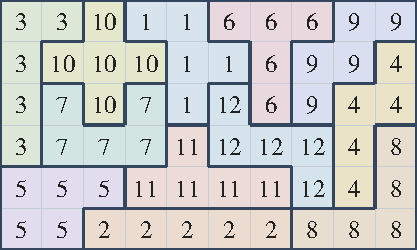
\includegraphics[height=31mm]{figures/csp-6x10.pdf}
    \caption{$6\times10$ board}
  \end{subfigure}\hfill
  \begin{subfigure}[t]{.47\linewidth}
    \centering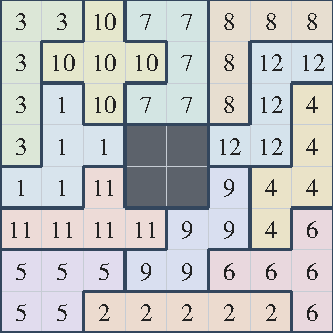
\includegraphics[height=31mm]{figures/csp-hole.pdf}
    \caption{Board with a central hole}
  \end{subfigure}
  \caption{Pentomino tilings. Equal labels identify cells belonging to one tile.}
\end{figure}

\clearpage
\section{Section II\quad Predefined Agents}
\subsection{Rules and search settings}
The game ends when either player first completes a line on any local board.
Local boards are indexed from 0 to 8 in row-major order. A move's position
within its local board determines the opponent's next local board. If that
board is full, the opponent may choose any empty global cell. All four games
start on board 4. Offensive X moves first in games 1--2; defensive O moves
first in games 3--4.

The predefined evaluation has three ordered tiers. Terminal states receive
10000 for an X win and $-10000$ for an O win. Otherwise, X scores 500 per
unblocked two-in-a-row and 100 per blocked O two-in-a-row. O scores $-100$
per unblocked two-in-a-row and $-500$ per blocked X two-in-a-row. Only when
the second tier has no counts are occupied local corners scored: 30 each
for X and $-30$ each for O. Rows, columns, and diagonals are counted
separately, so a cell may contribute to more than one line.

Both algorithms search three plies and stop early at terminal states.
Leaves use the root agent's evaluation throughout a search, always expressed
as X utility: X maximizes and O minimizes. Moves are visited in row-major
order, and the current best move is replaced only by a strict improvement.
Thus ties retain the first move. Alpha--beta search prunes when
$\alpha\geq\beta$.

\subsection{Outcomes and pruning}
Node counts include visited roots and leaves and are summed over all turns.
In Table~\ref{tab:predefined}, MM denotes minimax and AB denotes alpha--beta.
\begin{table}[htbp]
  \centering\small
  \caption{Results of the four required matchups.}\label{tab:predefined}
  \begin{tabular}{ccccrrrrc}
\toprule
Game & X & O & First & Plies & X nodes & O nodes & Total & Win \\
\midrule
1 & MM & MM & X & 43 & 8768 & 7948 & 16716 & X \\
2 & MM & AB & X & 43 & 8768 & 3398 & 12166 & X \\
3 & AB & MM & O & 44 & 3353 & 8528 & 11881 & X \\
4 & AB & AB & O & 44 & 3353 & 3431 & 6784 & X \\
\bottomrule
\end{tabular}

\end{table}

X won all four games. Games 1--2 have identical move sequences, with a
\PruningReductionA{} reduction in visited nodes after pruning. Games 3--4
also have identical sequences, with a \PruningReductionB{} reduction.
Alpha--beta therefore preserved minimax decisions while reducing search
effort in these matchups. Games 1 and 4 cannot isolate the effect of pruning
because they have different starting players.

The offensive heuristic emphasizes creating its own threats, whereas the
defensive heuristic emphasizes completed blocks. The latter does not
directly measure the danger of the board to which the next player is sent,
which can leave it vulnerable to sequences of forced routing.
\clearpage
\subsection{Final boards}
\begin{figure}[htbp]
\centering
\begin{subfigure}[t]{.46\linewidth}
\centering
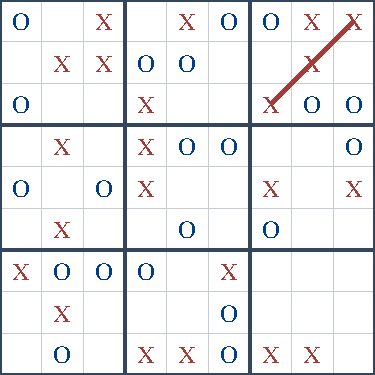
\includegraphics[height=48mm]{figures/predefined-1.pdf}
\caption{Game 1: X wins; 16,716 nodes}
\end{subfigure}
\hfill
\begin{subfigure}[t]{.46\linewidth}
\centering
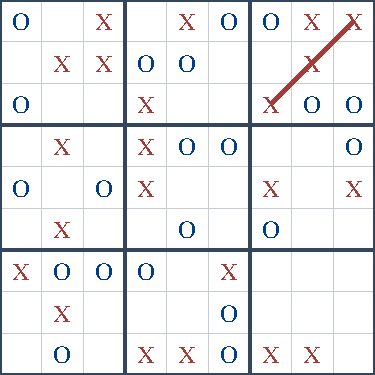
\includegraphics[height=48mm]{figures/predefined-2.pdf}
\caption{Game 2: X wins; 12,166 nodes}
\end{subfigure}
\par\medskip
\begin{subfigure}[t]{.46\linewidth}
\centering
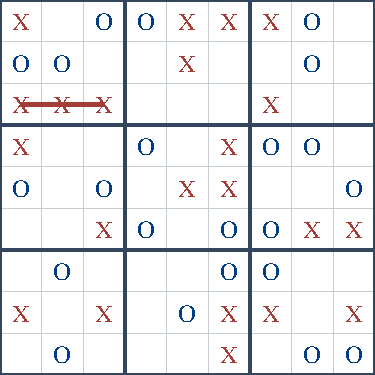
\includegraphics[height=48mm]{figures/predefined-3.pdf}
\caption{Game 3: X wins; 11,881 nodes}
\end{subfigure}
\hfill
\begin{subfigure}[t]{.46\linewidth}
\centering
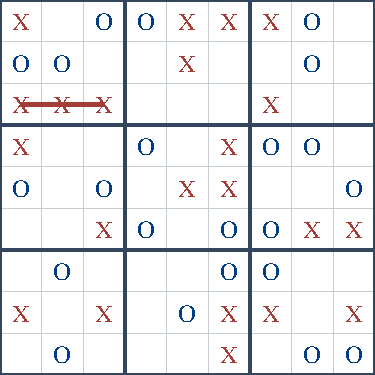
\includegraphics[height=48mm]{figures/predefined-4.pdf}
\caption{Game 4: X wins; 6,784 nodes}
\end{subfigure}
\caption{Final boards of the predefined agents.}
\end{figure}

\noindent\small X is offensive and O is defensive. Thick lines separate local
boards; colored lines mark winning triples. The four boards correspond to
the rows of Table~\ref{tab:predefined}.\normalsize

\clearpage
\section{Section III\quad Designed Evaluation}
\subsection{Formulation}
The designed agent plays O against predefined offensive X. Both use
depth-three alpha--beta search. The evaluation considers both players'
threats and the board where the next player must actually move. A winning
opportunity elsewhere is not necessarily playable on the next turn, so
routing is evaluated explicitly.

Let $T$ count unblocked two-in-a-row lines, $W$ sum distinct winning empty
cells over local boards, and $F$ count local boards with at least two
distinct winning cells. Let $C$ count occupied corners and $M$ occupied
centers, with subscripts X and O identifying the player. Set $s=1$ when X
moves next and $s=-1$ when O moves next. Of the next player's $L$ legal
moves, $S$ are safe: they do not immediately send the opponent to a board
where that opponent can win. When a move routes back to the same local
board, its cell is updated before testing the danger.
\begin{align*}
H={}&400(T_X-T_O)+35(W_X-W_O)+800(F_X-F_O)\\
   &+15(C_X-C_O)+40(M_X-M_O)+6000s\frac{S}{L}.
\end{align*}

Actual terminal states take priority and return $\pm10000$. If the next
player can win immediately, return $9500s$. If every legal move allows an
immediate opponent win, return $-9000s$. Otherwise, use $H$ clipped to
$[-8000,8000]$. A full global board with no winner returns zero. These
static tactical checks do not extend the recursive search beyond three plies.

The ratio $S/L$ avoids favoring a board merely because it has fewer empty
cells. The feature $F$ distinguishes two independent winning cells from
two lines sharing one blocking cell. Immediate threats take priority over
general positional scores; centers and corners have smaller weights.

\subsection{Parameter comparison}
Development covered all nine starting boards and both starting players,
giving eighteen conditions. The initial safe-count scheme won eleven;
the best adjusted safe-count scheme won fourteen. Position weights,
threat spread, and safety ratios were then compared. The ratio weight
6000 was selected for the most development wins in Table~\ref{tab:tuning}.
\begin{table}[htbp]
  \centering\small
  \caption{Development comparison of mobility features.}\label{tab:tuning}
  \begin{tabular}{lrr}
\toprule
Mobility feature & Weight & Development wins / 18 \\
\midrule
Safe-move count & 35 & 11 \\
Safe-move count & 1000 & 14 \\
Safe-move ratio & 1000 & 16 \\
Safe-move ratio & 3000 & 16 \\
Safe-move ratio & 6000 & 18 \\
\bottomrule
\end{tabular}

\end{table}

There are only eighteen opening conditions, so development and subsequent
random games are not strictly independent. The results establish an
improvement against this specified opponent, rather than a guarantee
against arbitrary strategies.

\clearpage
\subsection{Randomized match results}
With random seed 448, each game's starting board and player were sampled
randomly. Across \DesignedGames{} games, O won \DesignedWins{}, X won
\DesignedLosses{}, and \DesignedDraws{} were drawn. The designed agent's
win rate was \DesignedWinRate{}, exceeding the required 80\%.
The average total search count was \DesignedMeanNodes{} nodes per game.
\begin{table}[htbp]
  \centering\small
  \caption{Per-game results; node counts sum both players' searches.}\label{tab:random}
  \begin{minipage}[t]{.48\linewidth}\centering
    \begin{tabular}{ccccrc}
\toprule
Game & Start & First & Plies & Nodes & Win \\
\midrule
1 & 4 & O & 33 & 5,759 & O \\
2 & 1 & X & 36 & 7,901 & O \\
3 & 4 & O & 33 & 5,759 & O \\
4 & 0 & X & 32 & 6,700 & O \\
5 & 8 & O & 27 & 5,217 & O \\
6 & 6 & X & 36 & 7,107 & O \\
7 & 1 & X & 36 & 7,901 & O \\
8 & 3 & X & 38 & 6,716 & O \\
9 & 8 & O & 27 & 5,217 & O \\
10 & 5 & X & 36 & 6,536 & O \\
11 & 5 & O & 41 & 6,969 & O \\
12 & 7 & X & 36 & 6,206 & O \\
13 & 4 & X & 34 & 6,104 & O \\
14 & 8 & O & 27 & 5,217 & O \\
15 & 5 & O & 41 & 6,969 & O \\
16 & 5 & X & 36 & 6,536 & O \\
17 & 1 & X & 36 & 7,901 & O \\
18 & 0 & X & 32 & 6,700 & O \\
19 & 0 & O & 35 & 7,409 & O \\
20 & 5 & X & 36 & 6,536 & O \\
\bottomrule
\end{tabular}

  \end{minipage}\hfill
  \begin{minipage}[t]{.48\linewidth}\centering
    \begin{tabular}{ccccrc}
\toprule
Game & Start & First & Plies & Nodes & Win \\
\midrule
21 & 3 & X & 38 & 6,716 & O \\
22 & 8 & O & 27 & 5,217 & O \\
23 & 3 & O & 29 & 5,976 & O \\
24 & 8 & O & 27 & 5,217 & O \\
25 & 4 & X & 34 & 6,104 & O \\
26 & 6 & X & 36 & 7,107 & O \\
27 & 6 & O & 37 & 7,187 & O \\
28 & 7 & X & 36 & 6,206 & O \\
29 & 6 & O & 37 & 7,187 & O \\
30 & 1 & O & 33 & 6,850 & O \\
31 & 6 & O & 37 & 7,187 & O \\
32 & 5 & X & 36 & 6,536 & O \\
33 & 3 & O & 29 & 5,976 & O \\
34 & 0 & X & 32 & 6,700 & O \\
35 & 6 & X & 36 & 7,107 & O \\
36 & 3 & X & 38 & 6,716 & O \\
37 & 0 & O & 35 & 7,409 & O \\
38 & 8 & O & 27 & 5,217 & O \\
39 & 3 & O & 29 & 5,976 & O \\
40 & 3 & X & 38 & 6,716 & O \\
\bottomrule
\end{tabular}

  \end{minipage}
\end{table}

Policies and tie-breaking are deterministic. Repeated starting conditions
therefore produce repeated games; the forty runs are not forty distinct
tests of opponent strategy.

\clearpage
\subsection{Representative positions}
\begin{figure}[htbp]
\centering
\begin{subfigure}[t]{.46\linewidth}
\centering
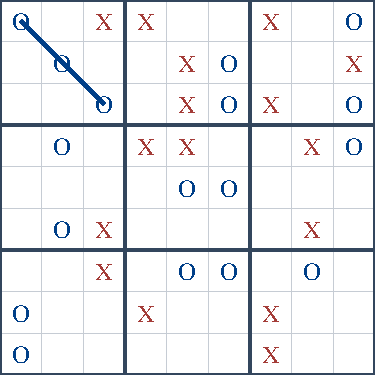
\includegraphics[height=48mm]{figures/designed-1.pdf}
\caption{Game 1: start 4, O first}
\end{subfigure}
\hfill
\begin{subfigure}[t]{.46\linewidth}
\centering
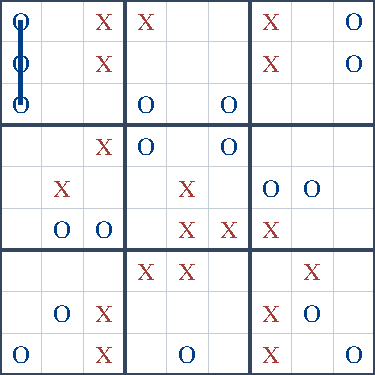
\includegraphics[height=48mm]{figures/designed-2.pdf}
\caption{Game 2: start 1, X first}
\end{subfigure}
\par\medskip
\begin{subfigure}[t]{.46\linewidth}
\centering
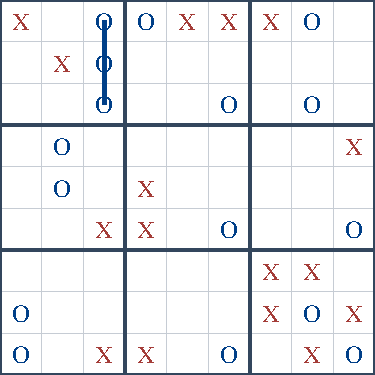
\includegraphics[height=48mm]{figures/designed-3.pdf}
\caption{Game 4: start 0, X first}
\end{subfigure}
\hfill
\begin{subfigure}[t]{.46\linewidth}
\centering
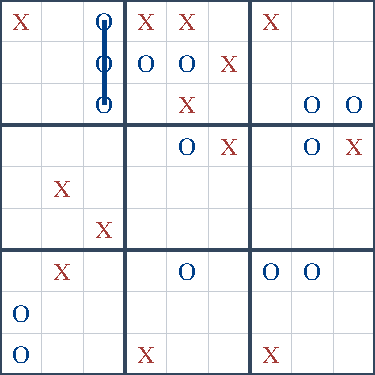
\includegraphics[height=48mm]{figures/designed-4.pdf}
\caption{Game 5: start 8, O first}
\end{subfigure}
\caption{Representative final boards of the designed agent.}
\end{figure}

Immediately before the final move, X had 5, 7, 3, 4 legal choices in the four games, respectively, but none could prevent O from winning on the next turn. The preceding threats and routing had already forced the outcome; these wins did not merely depend on X overlooking a final block.

The predefined offensive agent emphasizes its own two-in-a-row score,
whereas the designed evaluation also considers the destination of the next
turn and gives routing threats greater priority. Final boards alone cannot
isolate the causal effect of an individual weight. These findings remain
specific to the tested opponent and opening conditions.

\clearpage
\section{Section IV\quad Human Games}
The human plays X and the designed agent plays O, with randomized starting
board and player. At least ten games are required, followed by a discussion
of win rates, representative final boards, and the agent's strengths and weaknesses.
This section is a data-entry layout. The tables and reserved boards contain no measured games; dashes do not mean draws or zero win rates.


Depth-three search can miss longer forced-routing sequences. The safety
ratio checks immediate danger, not safety across several future turns.
Human games should examine whether threats prepared on several boards can
force the agent into an unavoidable loss, and whether fixed corner and
center weights interfere with necessary defense. These are questions for
the planned experiment, not empirical conclusions from human play.

\section{Extra Credit}
The global three-board-in-a-row extension was not implemented.

\section{Statement of Contribution}
The following is a proposed allocation for distributing the remaining work,
not a record of completed individual contributions. The group should
review the results together and update this statement after completing
the assigned tasks.

\begin{table}[htbp]
  \centering\small
  \caption{Proposed allocation, pending group confirmation.}
  \renewcommand{\arraystretch}{1.25}
  \begin{tabular}{lp{110mm}}
    \toprule
    Member & Proposed responsibility\\
    \midrule
    Wang Libin & CSP formulation, tiling solver review, correctness checks, and Section I.\\
    Jiang Jiahao & Minimax and alpha--beta review, four predefined matchups, node statistics, and Section II.\\
    Wang Zizheng & Designed evaluation, parameter comparison, randomized game analysis, and Section III.\\
    Xue Xiaokang & Organizing at least ten human games, recording representative boards, Section IV, and coordinating proofreading.\\
    \bottomrule
  \end{tabular}
\end{table}

The current code, automated experiments, and report draft were prepared
with Codex assistance.
\end{document}
